\section{3D Skeleton Prediction}

The first class of techniques, known as \textit{skeletal prediction} methods, output sets of either 2D or 3D keypoint locations. Since only a skeleton outline is obtained, apart from basic limb measurements, no other shape detail (e.g. surface definition, object density etc.) is obtained. However, it should be noted that this output form is often perfectly satisfactory depending on the intended application. In particular, this family of techniques have found numerous applications in controllerless gaming (e.g. Microsoft Kinect~\cite{kinectpaper}), motion capture (e.g. for digital character generation~\cite{xxx}), gait analysis (e.g. identifying lameness in cattle~\cite{xxx}) and many more. 

Early approaches in this category build statistical models of limb lengths and poses using freely available motion capture data~\cite{barron2001estimating}. These are then used to adapt a digital skeleton to fit each frame of an input video sequence.  

\subsection{Kinect skeletal tracking}
Shotton et al.~\cite{kinectpaper} designed a human skeletal tracking capability, which was later incorporated into the Microsoft Kinect Sensor SDK (see Figure \ref{fig:kinect_skeleton}. A large motion capture database containing approximately 500K frames was captured from human subjects performing a wide variety of activities (e.g.\ driving, dancing, kicking, running, etc.). This dataset was then used to drive a generative body model (constituting strong prior knowledge for this problem) which could be sampled from to create synthetic depth images with dense body part labels. A random forest classifier is then used to predict these body labels on unseen examples. A per-pixel density estimator for each body part is calculated for each 3D world space coordinate based on: (1) the inferred body part probability for the projected pixel, (2) the world surface area of the pixel. Density estimators for each body part are then used in combination to localize particular body joints, which are annotated with a calculated confidence value. 

\begin{figure}[H] % Example image
    \center{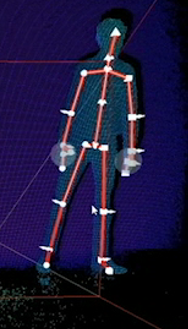
\includegraphics[width=0.25\linewidth]{human_tracking}}
    \caption{Kinect generating per-pixel joint proposals.}
    \label{fig:kinect_skeleton}
\end{figure}

\subsection{Multi-stage approaches}
More recent approaches are either predict 2D joint positions on an input image, and use a subsequent step that `lifts' these to a 3D pose, or predicts the 3D pose directly. Note that both approaches must overcome significant ambiguity. Determining joint positions is a task made challenging due to large variations in visual appearence, commonly due to clothing, body shape and camera view. As explained by Toshev and Szegedy~\cite{toshev2014deeppose}, even with perfect joint locations the subsequent lifting step is also ill-posed, as the space of consistent 3D poses for given 2D landmark locations is infinite. This is typically resolved using strong prior knowledge which usually takes the form of 3D geometric pose priors and temporal or structural constraints. Examples of such systems include DeepPose~\cite{toshev2014deeppose}, an approach which employs a CNN to reason jointly about 2D landmark detection and 3D pose estimation from single RGB images. Pishchulin et al.~\cite{pishchulin2016deepcut} later introduced DeepCut which extends DeepPose to the multi-person case. Both systems are trained on large body joint databases. 

\subsection{Direct approaches}
However, some direct techniques exist which do not require an initial 2D joint prediction. These include methods that directly regress to a 3D pose~\cite{tekin2016direct}. However, these typically rely on an annotated set of 3D joint labels, which can be difficult and costly to obtain, or being able to build a representative synthetic dataset, which is non-trivial task.



\subsection{More stuff}
There is an extensive body of prior work related to joint position prediction for human subjects. Earlier work used graphical approaches such as pictorial structure models~\cite{andriluka2010monocular,pishchulin2013poselet,johnson2010clustered}, which have since been replaced with deep learning-based methods~\cite{cao2017realtime,bulat2016human}. Few works predict animal joint positions directly owing to the lack of annotated data, although Mathis {\em et al.}~\cite{mathis2018deeplabcut} demonstrate the effectiveness of human pose estimation architectures for restricted animal domains. Our method instead trains on silhouette input, allowing the use of synthetic training imagery. The related task of animal part segmentation~\cite{wang2015joint,wang2015semantic} has seen some progress due to general object part datasets~\cite{chen_cvpr14,zhou2017scene}.

%% Discuss Amazon's system, Novotny's system etc.

\subsection{Applicability to animal categories}
% 2D predictor DeepLabCut 

